\documentclass[a4paper, 12pt]{article}
\usepackage[utf8]{inputenc}
\usepackage[brazil]{babel}
\usepackage{amstext} 	% need for \text command
\usepackage{amsmath}    % need for subequations
\usepackage{amssymb}
\usepackage{graphicx}   % need for figures
\usepackage{verbatim}   % useful for program listings
\usepackage{color}      % use if color is used in text
\usepackage{subfigure}  % use for side-by-side figures
\usepackage{hyperref}   % use for hypertext links, including those to external documents and URLs
\usepackage{pictexwd}	% use for pictex graphs
\usepackage{booktabs}	% use for Publication quality tables in LaTeX
\usepackage{lipsum}

\title{PME2321 - Exercicio}
\author{Vítor Matosinho Martins \\ 
nº USP:\ \ 5463225 \\
Prof Mauricio}

\begin{document}
\maketitle
%\newpage
%\tableofcontents
%\newpage

\section{Exercício 1 Lista Ciclos}
Um ciclo de turbina a gás, para uso veicular, é formado por um compressor e duas
turbinas. O ar (temperatura $T_{1}$=300 K e pressão $P_{1}$ = 100 kPa) entra no compressor ($\eta _{c}$ = 0,83) e sai com pressão $P_{2}$=500 kPa. Após passar pelo regenerador ($\eta _{r}$ = 0,8) (temperatura de saída $T_{3}$) e pelo combustor (temperatura de saída $T_{4}$ = 1600 K), o ar entra na primeira turbina, saindo com pressão $P_{5}$ , apenas o suficiente para que a turbina acione o compressor. O gás é então expandido numa segunda turbina, que aciona as rodas motrizes, passa pelo regenerador e é descarregado na atmosfera, com $P_{7}$ = 100 kPa. A vazão mássica de ar é de 0,6 kg/s e a eficiência das duas turbinas é de $\eta _{t}$ = 0,88. Sabendo-se que as propriedades do ar e dos gases de combustão podem ser considerados constantes e iguais ao do ar frio, determine:

\begin{figure}[h]
\begin{center}
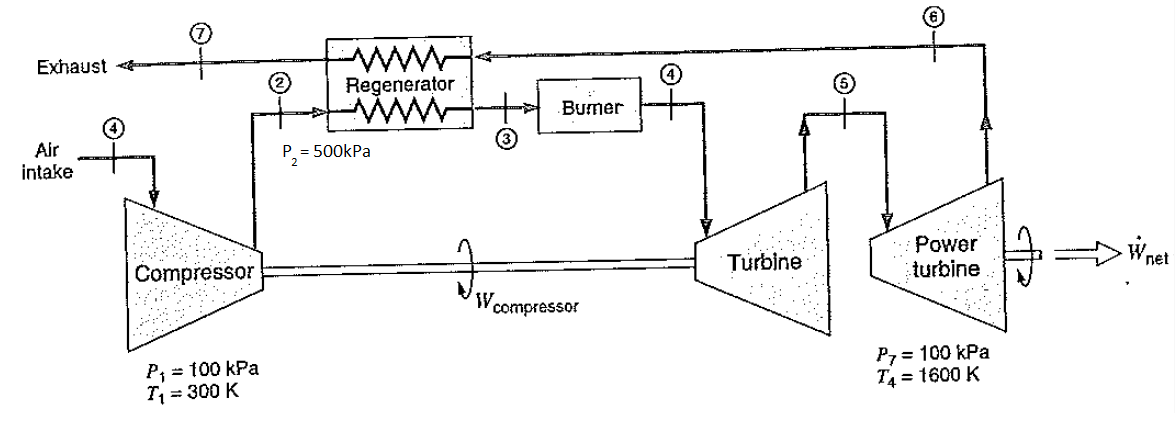
\includegraphics[scale=0.43,angle=-1.2]{./fig/1.png}
\caption{\label{fig:1}Ciclo Brayton} 
\end{center}
\end{figure}

\pagebreak

Usaremos calores específicos constantes na resolução

\subsection{a}
\paragraph*{Temperatura do ar na saída do compressor}

\begin{itemize}
\item $T_{1}$ = 300 K
\item $P_{1}$ = 100 kPa
\item $P_{2}$ = 500 kPa
\item k = 1.4
\end{itemize}

Considerando um compressor ideal (isentrópico)

\[\left( \frac{T_{2S}}{T_{1}}   \right) = \left( \frac{P_{2}}{P_{1}} \right)^{\frac{k-1}{k}} \]

\[T_{2S} = 475.146 K\]
Agora, considerando o compressor com rendimento de 0.83, temos:
\[\eta _{C} = \frac{W_{s}}{W} = \frac{T_{1} - T_{2S}}{T_{1} - T_{2}}\]
\[T_{2} = T_{1} - \frac{T_{1}-T_{2s}}{\eta} = 300 - \frac{(300-475)}{0.83}\]
\[T_{2} = 510.84 K\]

\subsection{b}
\paragraph*{A pressão intermediária $p_{5}$}
Estamos interessados na pressão $p_{5}$ do ciclo, que pode ser obtida usando a relação:

\begin{equation}
\left( \frac{T_{5s}}{T_{4}}   \right) = \left( \frac{P_{5}}{P_{4}} \right)^{\frac{k-1}{k}} 
\label{eq:1}
\end{equation}


Para isso precisamos obter antes $T_{5s}$, $T_{4}$ e $P_{4}$. Sabemos que:

\begin{itemize}
\item $T_{4}$ = 1600 K (do enunciado)
\item $P_{4}$ = $P_{3}$ = $P_{2}$ = 500 kPa (combustor e regenerador operam à mesma pressão que o compressor $C_{1}$)
\end{itemize}

$T_{5,s}$ pode ser obtida através de $w_{T1,s} = Cp_{0}(T_{5,s}-T_{4})$, em que:
\[\frac{w_{T1}}{w_{T1,s}} = \eta _{T1}  \]
\[\frac{w_{T1}}{ \eta _{T1} } =  w_{T1,s}   \]

E $w_{T1}$ pode ser obtida usando a relação:
\[ w_{T1} = -w_{C} \]
Mas 
\[w_{C} = -Cp_{0}(T_{2}-T_{1})\]
Logo,
\[w_{T1} = Cp_{0}(T_{2}-T_{1})\]
\[\frac{Cp_{0}(T_{2}-T_{1})}{ \eta _{T1} } =  Cp_{0}(T_{5,s}-T_{4})  \]

\[T_{5,s} = T_{4} + \frac{(T_{2}-T_{1})}{ \eta _{T1} } = 1600 + \frac{(510.84-300)}{ 0.88 } = 1360.206 \ K \]

Substituindo $T_{5,s}$ na equaçao \ref{eq:1}:

\[\left( \frac{1360}{1600}   \right) = \left( \frac{P_{5}}{500} \right)^{\frac{1.4-1}{1.4}} \]
\[P_{5} = 283.247 \ MPa\]

\subsection{c}
\paragraph*{Trabalho líquido do motor}

\begin{equation}
\dot{W}_{T2} = \dot{m}Cp_{0}(T_{5}-T_{6})
\label{eq:3}
\end{equation}

Em que:
\begin{itemize}
\item $\dot{m}$ = 0.6 kg/s
\item $Cp_{0}$ = 1.004
\end{itemize}

Para obter $T_{5}$, usaremos a relação:

\[\eta _{T1} = \frac{(T_{5}-T_{4})}{(T_{5,s}-T_{4})}\]
Logo:
\[ T_{5}  = T_{4} + \eta _{T1}(T_{5,s}-T_{4}) = 1600 + 0.88(1360.2-1600)\]
\[T_{5} = 1388.976 \ K\]

Para obter $T_{6}$, usaremos a relação:

\begin{equation}
\eta _{T2} = \frac{(T_{6}-T_{5})}{(T_{6,s}-T_{5})}
\label{eq:2}
\end{equation}

Em que $T_{6,s}$ é obtida por:

\[\left( \frac{T_{6s}}{T_{5}}   \right) = \left( \frac{P_{6} = P_{7}}{P_{5}} \right)^{\frac{k-1}{k}} = \left( \frac{T_{6s}}{1388.976}   \right) = \left( \frac{100}{283.247} \right)^{\frac{1.4-1}{1.4}} \]
\[T_{6,s} = 1031.584 \ K\]

Substituindo $T_{6,s}$ na equaçao \ref{eq:2}:

\[ T_{6}  = T_{5} + \eta _{T2}(T_{6,s}-T_{5}) = 1388.976 + 0.88(1031.58-1388.976)\]
\[T_{6} = 1074.4707 \ K\]

Substituindo $T_{5}$ e $T_{6}$ na equação \ref{eq:3}

\[\dot{W}_{T2} = 0.6 \times 1.004 \times (1388.976 -1074.4707)\]
\[\dot{W}_{T2} = 189.46 \ kW\]

\subsection{d}
\paragraph*{A temperatura do ar na entrada do combustor}

Para encontrar $T_{3}$, usaremos a relação do rendimento no regenerador:

\[\eta _{r} = \frac{(T_{3}-T_{2})}{(T_{6}-T_{2})}\]

\[T_{3} =  T_{2} + \eta _{r}(T_{6}-T_{2}) = 510.84 + 0.8(1074.4707-510.84) \]
\[T_{3} = 961.7446 \ K\]

\subsection{e}

\[T_{7} = T_{6}- (T_{3}-T_{2})\]
\[T_{7} = 612.6 K\]

\paragraph*{O rendimento térmico do ciclo}

\[\eta _{ciclo} = \frac{W_{T1} + W_{T2} - W_{C}}{Q_{H}}\]
Sendo $W_{T1} = W_{C}$, temos:
\[\eta _{ciclo} = \frac{ W_{T2} }{Q_{H}} = \frac{188.703}{\dot{m}Cp_{0}(T_{4}-T_{3})}\]
\[\eta _{ciclo} = \frac{188.703}{0.6 \times 1.004 \times (1600 - 961.75)}\]
\[\eta _{ciclo} = 0.4908\]

\subsection{f}
\paragraph*{Diagrama Txs}

% Table generated by Excel2LaTeX from sheet 'Plan1'
\begin{table}[htbp]
  \centering
  \caption{Tabela de T por s}
    \begin{tabular}{rrrr}
    \toprule
    Estagio & P(MPa) & T(K)  & s(kJ/kg K) \\
    \midrule
    1     & 0,1   & 300   & 6,87 \\
    2     & 0,5   & 475,2 & 6,873 \\
    3     & 0,5   & 961,7446 & 7,628 \\
    4     & 0,5   & 1600  & 8,229 \\
    5     & 0,283247 & 1388,976 & 8,438 \\
    6     & 0,1   & 1031,584 & 8,445 \\
    7     & 0,1   & 612,6 & 7,998 \\
    \bottomrule
    \end{tabular}%
  \label{tab:1}%
\end{table}%

\begin{figure}[h]
\begin{center}
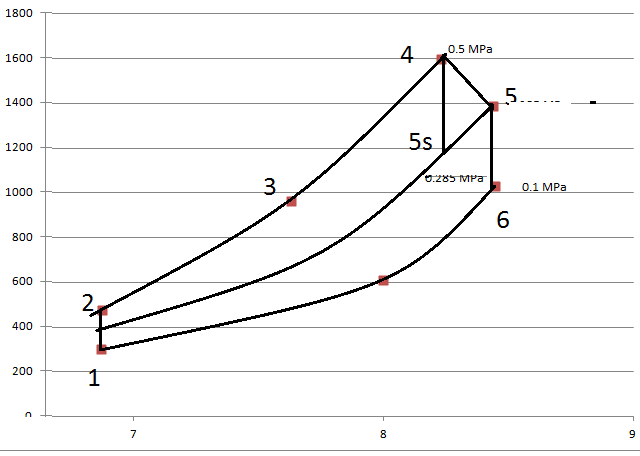
\includegraphics[scale=0.8,angle=-0.0]{./fig/2.png}
\caption{\label{fig:2}Diagrama T x s} 
\end{center}
\end{figure}

\end{document}